\documentclass{beamer}

\usetheme{metropolis}

\usepackage[ngerman]{babel}
\usepackage[autostyle=true,german=quotes]{csquotes}
\usepackage[linewidth=1pt]{mdframed}
\usepackage{hyperref}
\usepackage{makecell}
\usepackage{pifont}
\usepackage{tikz}
\usetikzlibrary{positioning, calc, arrows, fit, decorations.pathreplacing, shapes, shapes.multipart, snakes}
\usepackage{verbatim}
\usepackage{textcomp}
\usepackage{centernot}
\usepackage{tabularx}
\usepackage{ulem}
%\usepackage{pdfpages}

\batchmode

\hypersetup{
	colorlinks,
	urlcolor=blue,
	linkcolor=black % for ToC
}
\newenvironment{qaa}[1]{
	#1

	\begin{mdframed}
		\small
}{
	\end{mdframed}
}

\newcommand{\true}{\ding{51}}
\newcommand{\false}{\ding{55}}
\newcommand{\code}[1]{
	\begin{mdframed}
		\verbatiminput{#1}
	\end{mdframed}
}


\title{Tutorium 06: Prolog}
% \subtitle{}
\author{Paul Brinkmeier}
\institute{Tutorium Programmierparadigmen am KIT}
\date{15. Dezember 2020}

\begin{document}

\begin{frame}
	\titlepage
\end{frame}

\section{Heutiges Programm}

\begin{frame}{Programm}
	\begin{itemize}
		\item $\lambda$-Kalkül: Wiederholung
		\item Übungsblatt 4
                \item Aufgaben zu Prolog
	\end{itemize}
\end{frame}

\section{Wiederholung}

\begin{frame}{Cheatsheet: Lambda-Kalkül/Basics}
  \begin{itemize}
    \item Terme $t$: Variable ($x$), Funktion ($\lambda x . t$), Anwendung ($t \; t$)
    \item \emph{$\alpha$-Äquivalenz}: Gleiche Struktur
    \item \emph{$\eta$-Äquivalenz}: Unterversorgung
    \item \emph{Freie Variablen}, \emph{Substitution}, \emph{RedEx}
    \item \emph{$\beta$-Reduktion}: \\
          $(\lambda{}p.b)$ $t \Rightarrow b\left[p\rightarrow{}t\right]$
  \end{itemize}
\end{frame}


\begin{frame}{Cheatsheet: Lambda-Kalkül/Fortgeschritten}
  \begin{itemize}
    \item Auswertungsstrategien (von lässig nach streng):
    \begin{itemize}
      \item \emph{Volle $\beta$-Reduktion}
      \item \emph{Normalreihenfolge}
      \item \emph{Call-by-Name}
      \item \emph{Call-by-Value}
    \end{itemize}
    \item Datenstrukturen:
    \begin{itemize}
      \item \emph{Church-Booleans}
      \item \emph{Church-Zahlen}
      \item \emph{Church-Listen}
    \end{itemize}
    \item Rekursion durch \emph{Y-Kombinator}
  \end{itemize}
\end{frame}

\section{Übungsblatt 4}

\newcommand{\E}{\;}

\newcommand{\liin}[2]{#1\E{}#2}
\newcommand{\liiin}[3]{#1\E{}#2\E{}#3}
\newcommand{\livn}[4]{#1\E{}#2\E{}#3\E{}#4}
\newcommand{\lvn}[5]{#1\E{}#2\E{}#3\E{}#4\E{}#5}

\newcommand{\lii}[2]{(#1\E{}#2)}
\newcommand{\liii}[3]{(#1\E{}#2\E{}#3)}

\newcommand{\liir}[2]{\textcolor{red}{\underline{(}}#1\E{}#2\textcolor{red}{\underline{)}}}
\newcommand{\liiir}[3]{\textcolor{red}{\underline{(}}#1\E{}#2\E{}#3\textcolor{red}{\underline{)}}}

\newcommand{\abs}[2]{\lambda{}#1.#2}

\begin{frame}{1.1 --- Klammerung im $\lambda$-Kalkül}
	\footnotesize
	\begin{eqnarray}
		\liiin{c_0}{c_1}{\liii{c_2}{c_3}{c_4}}{c_5}                   =& \pause \liin{\liir{\liir{c_0}{c_1}}{\lii{\liir{c_2}{c_3}}{c_4}}}{c_5}             \\
		\liin{\liii{c_0}{c_1}{c_2}}{\liii{c_3}{c_4}{c_5}}             =& \pause \liin{\lii{\liir{c_0}{c_1}}{c_2}}{\lii{\liir{c_3}{c_4}}{c_5}}              \\
		\livn{c_0}{c_1}{\liii{c_2}{c_3}{c_4}}{\lii{c_5}{c_6}}         =& \pause \liin{\liir{\liir{c_0}{c_1}}{\lii{\liir{c_2}{c_3}}{c_4}}}{\lii{c_5}{c_6}}  \\
		\lvn{c_0}{c_1}{\liii{c_2}{c_3}{c_4}}{c_5}{c_6}                =& \pause \liin{\liir{\liir{\liir{c_0}{c_1}}{\lii{\liir{c_2}{c_3}}{c_4}}}{c_5}}{c_6} \\
		\livn{c_0}{\lii{c_1}{\liii{c_2}{c_3}{c_4}}}{c_5}{c_6}         =& \pause \liin{\liir{\liir{c_0}{\lii{c_1}{\lii{\liir{c_2}{c_3}}{c_4}}}}{c_5}}{c_6}  \\
		\liin{(\abs{y}{\liiin{c_0}{c_1}{c_2}})}{\liii{c_3}{c_4}{c_5}} =& \pause \liin{(\abs{y}{\liin{\liir{c_0}{c_1}}{c_2}})}{\lii{\liir{c_3}{c_4}}{c_5}}  \\
                \liin{(\abs{y}{\lii{c_0}{(\abs{z}{\lii{c_1}{c_2}})}})}{\liii{c_3}{c_4}{c_5}} =& \pause \liin{(\abs{y}{\lii{c_0}{(\abs{z}{\lii{c_1}{c_2}})}})}{\lii{\liir{c_3}{c_4}}{c_5}}
	\end{eqnarray}

	\normalsize
	\begin{itemize}
		\item Funktionsaufrufe sind linksassoziativ, wie in Haskell
		\item Bzw. in Haskell sind FA linksassoz., wie im $\lambda$-Kalkül
	\end{itemize}
\end{frame}

\setcounter{equation}{0}

\begin{frame}{1.2 --- Klammerung im $\lambda$-Kalkül}
	\begin{eqnarray}
		\liin{(\abs{y}{y})}{c_0} \stackrel{?}{=} \abs{y}{\liin{y}{c_0}} \\
		\abs{y}{\lii{y}{c_0}} \stackrel{?}{=} \abs{y}{\liin{y}{c_0}}
	\end{eqnarray}

      \only<1>{
        \begin{itemize}
                \item Term 1 $\approx$ \texttt{App (Abs "{}y"{} (Var "{}y"{})) (Var "{}c0"{})}
                \item Term 2 $\approx$ \texttt{Abs "{}y"{} (App (Var "{}y"{}) (Var "{}c0"{}))}
                \item $\leadsto$ zweite Gleichung stimmt
        \end{itemize}
      }
      \only<2>{
        \begin{itemize}
          \item Term 1 $\approx$ \texttt{app(abs(y, y), c0)}
          \item Term 2 $\approx$ \texttt{abs(y, app(y, c0))}
          \item $\leadsto$ zweite Gleichung stimmt
        \end{itemize}
      }

\end{frame}

\setcounter{equation}{0}

\begin{frame}{1.3 --- Klammerung im $\lambda$-Kalkül}
	\begin{eqnarray}
		\subst{\liin{(x)}{c_0}}{x}{\abs{y}{y}} =& \liin{(\abs{y}{y})}{c_0} \\
		\subst{\liin{x}{c_0}}{x}{(\abs{y}{y})} =& \liin{(\abs{y}{y})}{c_0} \\
		\subst{\liin{x}{c_0}}{x}{\abs{y}{y}} =& \liin{(\abs{y}{y})}{c_0}
	\end{eqnarray}

	\begin{itemize}
		\item Alle drei Substitutionen führen zum selben Ergebnis
		\item \enquote{Für beliebiges $t$ repräsentieren $t$ und $(t)$ den gleichen $\lambda$-Term} stimmt
	\end{itemize}
\end{frame}

\setcounter{equation}{0}

\begin{frame}{1.4 --- Klammerung im $\lambda$-Kalkül}
	Angenommen, $x = \liin{c_0}{c_1}$.\\
	Welche der folgenden Aussagen gelten?

	\begin{eqnarray}
		\liiin{c_0}{c_1}{c_2}                 =& \liin{x}{c_2} \\
		\liiin{c_2}{c_0}{c_1}                 =& \liin{c_2}{x} \\
		\livn{c_2}{\lii{c_3}{c_4}}{c_0}{c_1}  =& \liiin{c_2}{\lii{c_3}{c_4}}{x} \\
		\liin{c_2}{\liii{c_0}{c_1}{c_3}}{c_4} =& \liiin{c_2}{\lii{x}{c_3}}{c_4}
	\end{eqnarray}

	\pause

	\begin{itemize}
		\item 1 und 4 gelten
		\item $\liiin{c_2}{c_0}{c_1} = \liin{\liir{c_2}{c_0}}{c_1} \neq \liin{c_2}{\liir{c_0}{c_1}} = \liin{c_2}{x}$
		\item $\livn{c_2}{\lii{c_3}{c_4}}{c_0}{c_1} \stackrel{*}{\neq} \liiin{c_2}{\lii{c_3}{c_4}}{x}$
	\end{itemize}
\end{frame}

\section{Einführung in Prolog}

\begin{frame}{Prolog --- Umgebung}
  \begin{figure}
    
\includegraphics[width=0.25\textwidth]{images/swipl}
  \end{figure}
	\begin{itemize}
		\item Prolog ist eine Programmiersprache, wenn auch eine seltsame
		\item $\leadsto$ gut wird man durch Übung
		\item Zum Üben:
		\begin{itemize}
			\item SWI-Prolog --- gängige Prolog-Umgebung
			\item \href{https://swish.swi-prolog.org/}{SWISH} --- SWI-Prolog Web-IDE zum Testen
			\item VIPR, VIPER --- PSE-Tools des IPD, auf der \href{https://pp.ipd.kit.edu/lehre/WS202021/paradigmen/uebung/}{Seite der Übung} verlinkt
		\end{itemize}
	\end{itemize}
\end{frame}

\begin{frame}{Prolog --- Regelsysteme als Programmiersprache}
  \code{../demos/grandparents.pl}

  \vfill

  \only<1>{
    \texttt{?- grandparent(inge, kunibert).} $\leadsto$ \texttt{yes.}
  }

  \only<2>{
    \begin{mathpar}
      \inferrule{
        \inferrule{
          \inferrule{ }{\text{\texttt{mother(inge, emil)}}}
        }{
          \text{\texttt{parent(inge, emil)}}
        } \\
        \inferrule{
          \inferrule{ }{\text{\texttt{father(emil, kunibert)}}}
        }{
          \text{\texttt{parent(emil, kunibert)}}
        }
      }{
        \text{\texttt{grandparent(inge, kunibert)}}
      }
    \end{mathpar}
  }
\end{frame}

\begin{frame}{Funktoren}
	\code{../demos/funktoren.pl}

	\begin{itemize}
		\item Funktor $\approx$ Name + Liste von Prolog-Ausdrücken
		\item Liste leer $\leadsto$ \enquote{Atom}
		\item Name wird immer klein geschrieben
		\begin{itemize}
			\item Großbuchstaben: bspw. \texttt{'List'}
		\end{itemize}
                \item Auch mathematische Ausdrücke sind Funktoren:\\
                      \texttt{17 + 25} $\approx$ \texttt{'+'(17, 25)}
	\end{itemize}
\end{frame}

\begin{frame}{Variablen}
	\code{../demos/variablen.pl}

	\begin{itemize}
		\item Variablen werden immer groß geschrieben
		\item \texttt{=} ist nicht Zuweisung, sondern Unifikation
		\item Unifikation $\approx$ (formales) Pattern-Matching
	\end{itemize}
\end{frame}

\begin{frame}{Ziele}
	\code{../demos/ziele.pl}

	\begin{itemize}
		\item Funktionsaufruf $\approx$ \enquote{Zielerfüllung} in Prolog
		\item Mögliche Ziele:
		\begin{itemize}
			\item Unifikationsziel
                        \item \emph{Funktorziel}
			\item Arithmetische Zuweisung
			\item Arithmetischer Vergleich
			\item Nicht-Erfüllung
			\item Cut
		\end{itemize}
	\end{itemize}
\end{frame}

% Regeln: Kopf + [Ziel]
% Ziel: Funktor, Unifikation, Ungleichheit, Arithmetik

\begin{frame}{Programme}
	\begin{itemize}
		\item Prolog-\enquote{Programme} $\approx$ Datenbanken
		\item Ausführung $\approx$ Abfrage in der Datenbank
		\item Datenbank-Inhalt: Regeln, bestehend aus:
		\begin{itemize}
			\item Regelkopf --- Ein Funktor $\leadsto$ kann auch Atom sein
			\item Teilziele --- Liste von Zielen, um diese Regel zu erfüllen
			\item Keine Teilziele $\leadsto$ Fakt
		\end{itemize}
	\end{itemize}
\end{frame}

\section{Prolog-Aufgaben}

\subsection{Mathematiker-WG}

\begin{frame}{Mathematiker-WG}
	\begin{figure}
		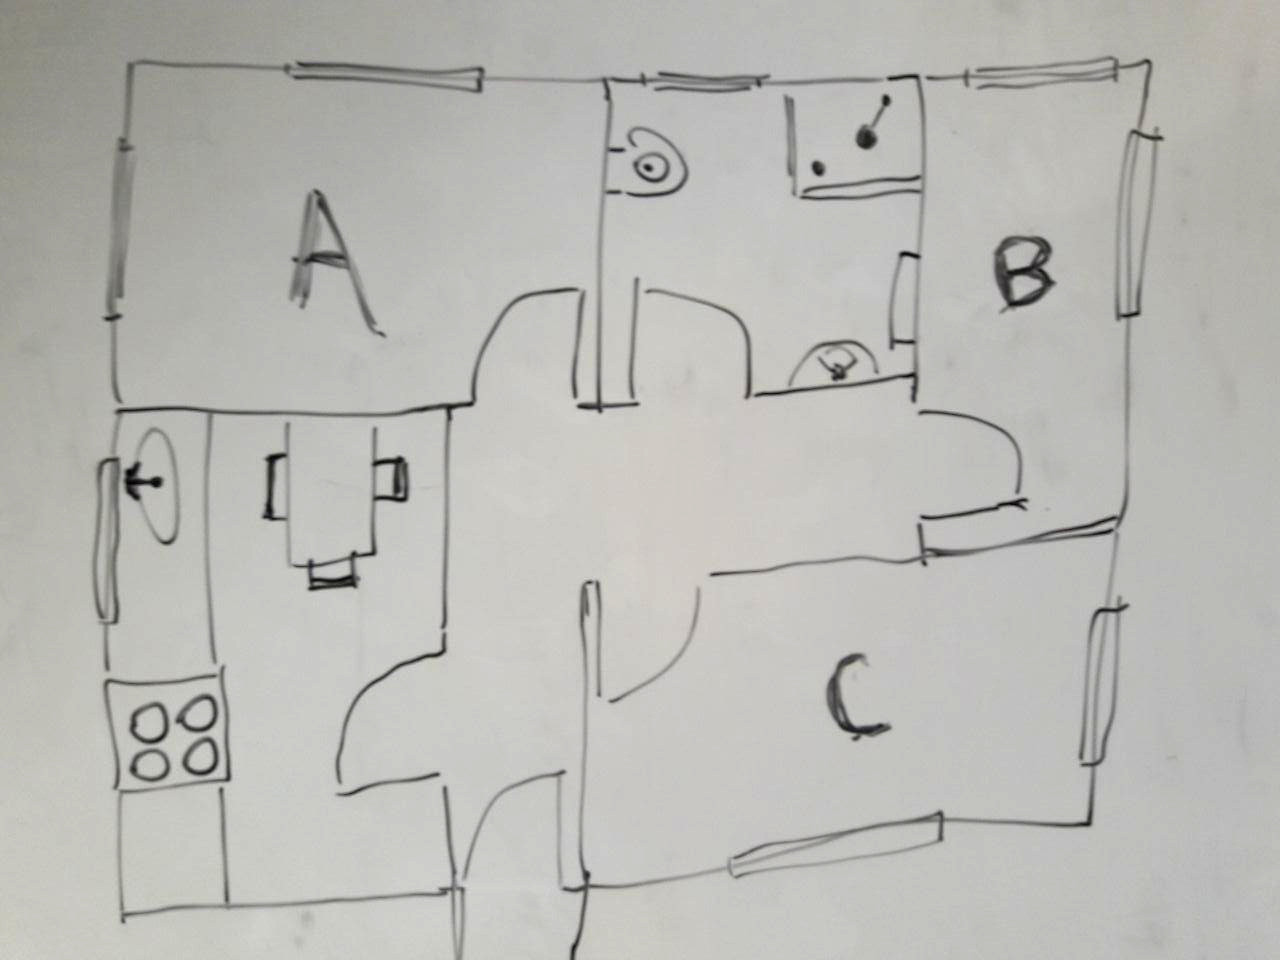
\includegraphics[width=0.8\textwidth]{images/mathematiker-wg}
	\end{figure}
\end{frame}

\begin{frame}{Mathematiker-WG}
	\begin{itemize}
		\item Alice, Bob und Carl ziehen in eine WG
		\item Die drei sind Mathematiker;\\jeder will eine eigene Zahl von 1 bis 7 für sein Zimmer
		\item Die Summe der Zahlen soll 12 sein
		\item Alice mag keine ungeraden Zahlen
	\end{itemize}

	Findet alle 14 möglichen Kombinationen, die Zimmer zu nummerieren.
\end{frame}

\begin{frame}{Mathematiker-WG}
	\code{../demos/mathematiker_wg.pl}
\end{frame}

\subsection{Detektivrätsel}

\begin{frame}{Detektivrätsel}
	\begin{figure}
		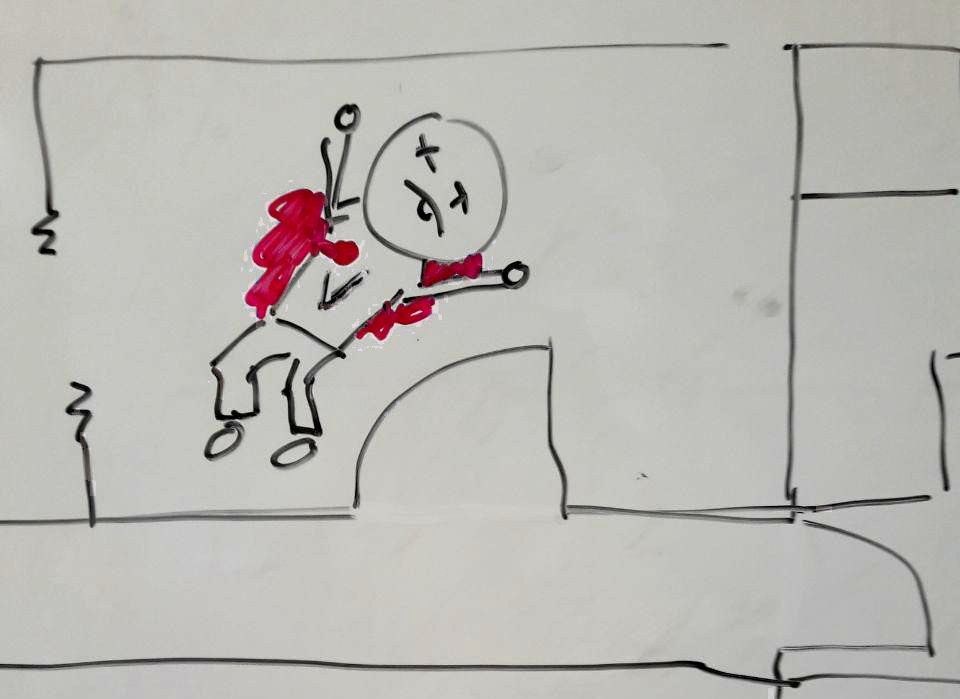
\includegraphics[width=0.8\textwidth]{images/victor}
	\end{figure}
\end{frame}

\begin{frame}{Detektivrätsel}
	Im Fall des Mordes an ihrem Nachbarn Victor sind nun Alice, Bob und Carl die einzigen Verdächtigen und Zeugen.
	\begin{itemize}
		\item Alice:
		\begin{itemize}
			\item Bob war mit dem Opfer befreundet.
			\item Carl und das Opfer waren verfeindet.
		\end{itemize}
		\item Bob:
		\begin{itemize}
			\item Ich war überhaupt nicht daheim!
			\item Ich kenne den garnicht!
		\end{itemize}
		\item Carl:
		\begin{itemize}
			\item Ich bin unschuldig!
			\item Wir waren zum Zeitpunkt der Tat alle in der WG.
		\end{itemize}
	\end{itemize}
\end{frame}

\begin{frame}{Detektivrätsel}
	\code{../demos/detektiv.pl}
\end{frame}

\begin{frame}{Detektivrätsel}
        \code{../demos/detektiv2.pl}
	
	\begin{itemize}
            \item \texttt{delete/3} wurde in der Vorlesung definiert.
            \item Implementiert: \texttt{inkonsistent/1}\\
                  Überprüft Aussagen von Zeugen paarweise auf Widerspruch
	\end{itemize}
\end{frame}

% aussage(alice, ...), aussage(bob, ...), jeweils freund, feind, fremder, daheim, unterwegs
% widerspruch
% select/3, oder selber implementieren
% inkonsistent(Liste), prüft ob paarweise widersprüche vorliegen

\subsection{Bettenverteilung}

\begin{frame}{Schlafplätze im Gefängnis}
	\begin{figure}
		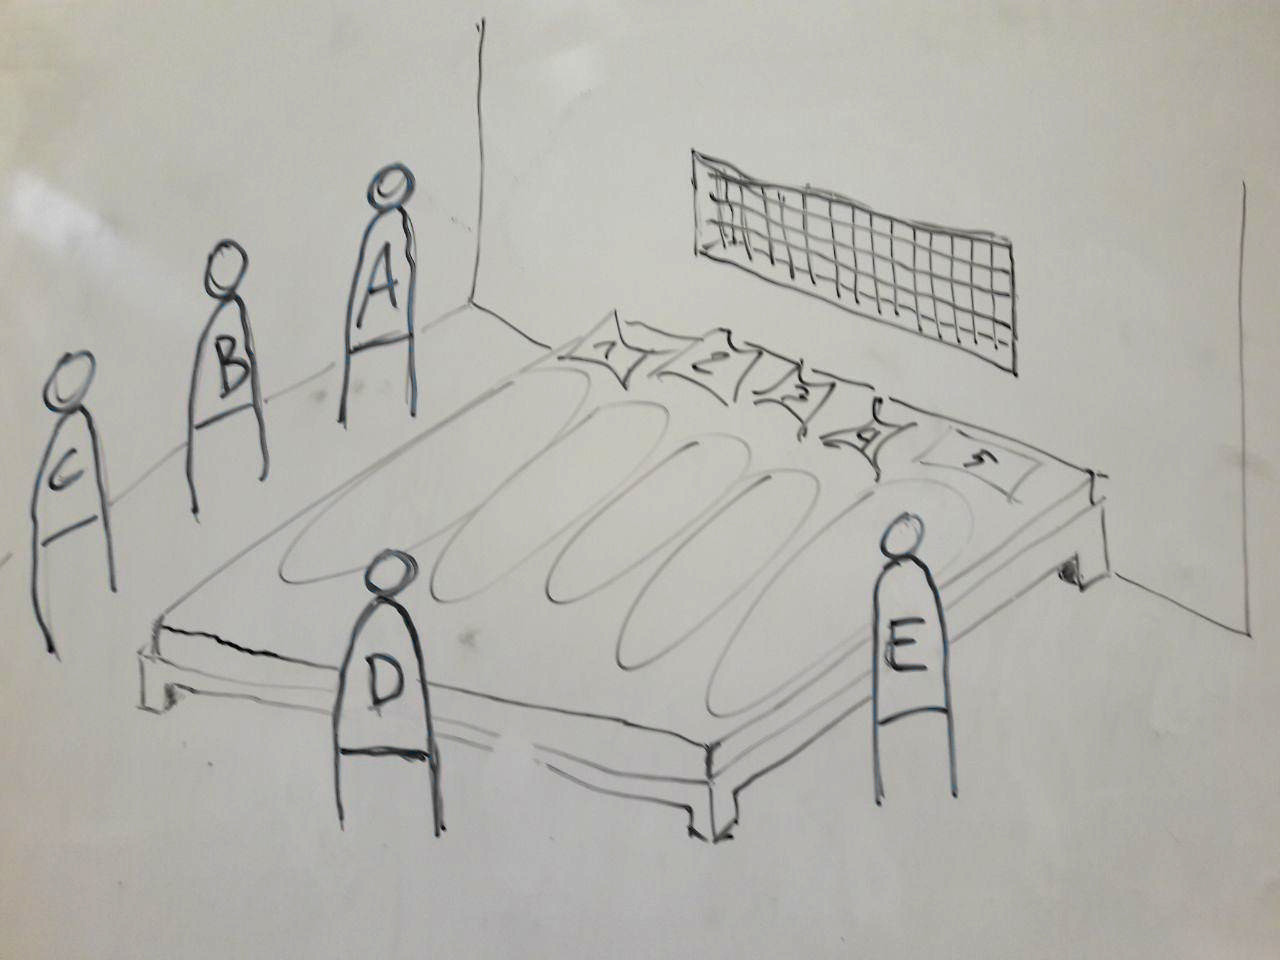
\includegraphics[width=0.8\textwidth]{images/bett}
	\end{figure}
\end{frame}

\begin{frame}{Dinesman's multiple-dwelling problem}
	Bob kommt nun ins Gefängnis.
	Aaron, Bob, Connor, David und Edison müssen sich zu fünft ein sehr breites Bett teilen.

	\begin{itemize}
		\item Aaron will nicht am rechten Ende liegen
		\item Bob will nicht am linken Ende liegen
		\item Connor will an keinem der beiden Enden liegen
		\item David will weiter rechts liegen als Bob
		\item Connor schnarcht sehr laut;\\Bob und Edison sind sehr geräuschempfindlich
		\begin{itemize}
			\item $\leadsto$ Bob will nicht direkt neben Connor liegen
			\item $\leadsto$ Edison will nicht direkt neben Connor liegen
		\end{itemize}
	\end{itemize}

	Wie können die 5 Schlafplätze verteilt werden?
\end{frame}

\begin{frame}{Schlafplätze im Gefängnis}
	\code{../demos/schlafplaetze.pl}

	\begin{itemize}
		\item Fügt weitere benötigte Tests ein
		\item Implementiert:
		\begin{itemize}
			\item \texttt{distinct/1} prüft Listenelemente auf paarweise Ungleichheit
			\item \texttt{adjacent/2} prüft, ob $|A - B| = 1$
		\end{itemize}
	\end{itemize}
\end{frame}

% ansatz: multipleDwelling(B, C, F, M, S) :- ....
% distinct/1
% adjacent/2

\begin{frame}{Putzdienst}
	\begin{figure}
		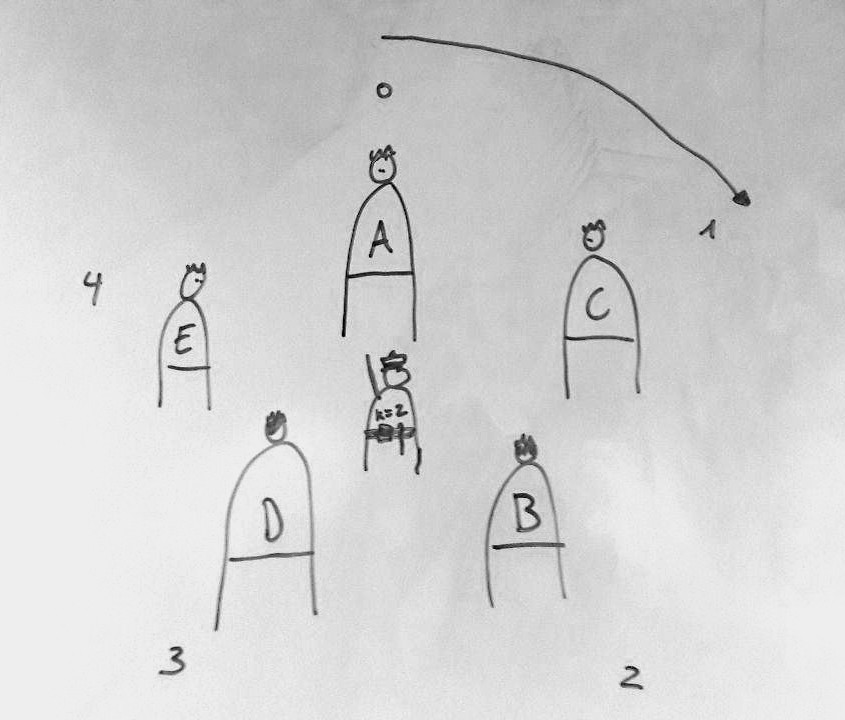
\includegraphics[width=0.7\textwidth]{images/putzdienst}
	\end{figure}
\end{frame}

\begin{frame}{Putzdienst}
	\begin{itemize}
		\item Aaron, Bob, Connor, David und Edison sollen 4 Einheiten Putzdienst übernehmen
		\item Da sie sich nicht einigen können, wer aussetzen darf, wendet ein Wärter folgendes Vorgehen an:
		\begin{itemize}
			\item Die fünf werden im Kreis aufgestellt
			\item Der Wärter stellt sich in die Mitte
			\item Beginnend bei 12 Uhr dreht er sich im Uhrzeigersinn und teilt jeden $k$-ten (bspw. $k = 2$) Insassen zum Putzdienst ein
			\begin{itemize}
				\item D.h. es werden immer $k - 1$ Insassen übersprungen
			\end{itemize}
		\end{itemize}
	\end{itemize}

	An welcher Stelle muss Bob stehen, um nicht putzen zu müssen?\\
	\pause
	An welcher Stelle muss Bob bei 41 Insassen und $k = 3$ stehen?
\end{frame}

\begin{frame}{Putzdienst}
	\code{../demos/putzdienst.pl}

	\begin{itemize}
		\item Weitere Fälle für \texttt{helper/4}:
		\begin{itemize}
			\item \texttt{C = 0} $\leadsto$ Element entfernen
			\item Ansonsten: Element hinten wieder anhängen
		\end{itemize}
	\end{itemize}
\end{frame}

\subsection{Quellen}

\begin{frame}{Quellen der Aufgaben}
	Zum Nachlesen und Vergleichen mit Lösungen in anderen Programmiersprachen:
	\begin{itemize}
		\item WG --- \href{https://rosettacode.org/wiki/Department_Numbers}{Rosetta Code: Department Numbers}
		\item Detektiv --- \href{https://github.com/Anniepoo/prolog-examples/blob/master/newdetective.pl}{github.com/Anniepoo/prolog-examples}
		\item Schlafplätze --- SICP, S. 418
		\item Putzdienst --- \href{https://rosettacode.org/wiki/Josephus_problem}{Rosetta Code: Josephus problem}
	\end{itemize}
\end{frame}

% quellen:
% multiple dwelling: SICP S. 418
% detective: https://github.com/Anniepoo/prolog-examples/blob/master/newdetective.pl
% department numbers: https://rosettacode.org/wiki/Department_Numbers
% josephus problem: https://rosettacode.org/wiki/Josephus_problem#Python


\end{document}
